% ============================================================
\chapter{The Mapper Algorithm}
\label{ch:mapper}
% ============================================================

In 2007, Gurjeet Singh, Facundo M\'emoli, and Gunnar Carlsson published a paper that would transform applied TDA: the Mapper algorithm. The idea is remarkably simple: instead of computing the persistent homology of a point cloud (which produces numerical invariants but no direct visualization), Mapper constructs a \emph{graph} that captures the global shape of the data. The procedure draws inspiration from the nerve theorem: one partitions the data into overlapping pieces using a filter function, clusters the points within each piece, then connects clusters that share points. The resulting graph is a ``map'' of the data, hence the name. Mapper has been used to discover a subgroup of breast cancer, analyse athletic performance, and explore genomic data --- wherever visualizing the ``shape'' of data provides insight inaccessible to classical statistical methods.

\begin{intuition}
Mapper is a topological visualization algorithm that constructs a
summary graph capturing the global structure of a high-dimensional
dataset. Unlike persistent homology which computes numerical invariants,
Mapper produces an interpretable geometric object.
\end{intuition}

% ============================================================
\section{Motivation}
% ============================================================

Dimensionality reduction techniques (PCA, t-SNE, UMAP) project data
into a low-dimensional space but inevitably lose structural information.
Mapper takes a different approach: it constructs a simplicial graph that
preserves topological properties of the dataset.

\begin{definition}[Reeb Graph --- Underlying Idea]
Let $f : X \to \R$ be a continuous function on a topological space $X$.
The \emph{Reeb graph} $\mathcal{R}_f(X)$ is the quotient of $X$ by the
relation: $x \sim y$ iff $f(x) = f(y)$ and $x, y$ are in the same
connected component of $f^{-1}(f(x))$.
\end{definition}

Mapper is a \emph{discrete approximation} of the Reeb graph.

% ============================================================
\section{The Mapper Algorithm}
% ============================================================

\begin{algorithme}[title=\textbf{Mapper Algorithm (Singh, M\'emoli, Carlsson, 2007)}]
\textbf{Inputs}: Point cloud $X$, filter function $f : X \to \R^k$,
cover $\mathcal{U}$ of $f(X)$, clustering algorithm $\mathcal{C}$.

\begin{enumerate}
  \item \textbf{Filtering}: apply $f$ to obtain $f(X) \subset \R^k$.
  \item \textbf{Covering}: choose a cover
        $\mathcal{U} = \{U_\alpha\}_{\alpha \in A}$ of $f(X)$ by open
        sets (typically overlapping intervals).
  \item \textbf{Pullback and clustering}: for each $U_\alpha$, compute
        $f^{-1}(U_\alpha) \cap X$ and apply clustering algorithm
        $\mathcal{C}$, yielding clusters
        $C_{\alpha,1}, \ldots, C_{\alpha, k_\alpha}$.
  \item \textbf{Nerve construction}: build the simplicial complex whose
        vertices are the clusters and where
        $\{C_{\alpha_0, i_0}, \ldots, C_{\alpha_p, i_p}\}$ forms a
        simplex iff
        $C_{\alpha_0, i_0} \cap \cdots \cap C_{\alpha_p, i_p} \neq \emptyset$.
\end{enumerate}
\textbf{Output}: the simplicial complex (often a graph, i.e., a
$1$-dimensional complex).
\end{algorithme}

\begin{center}
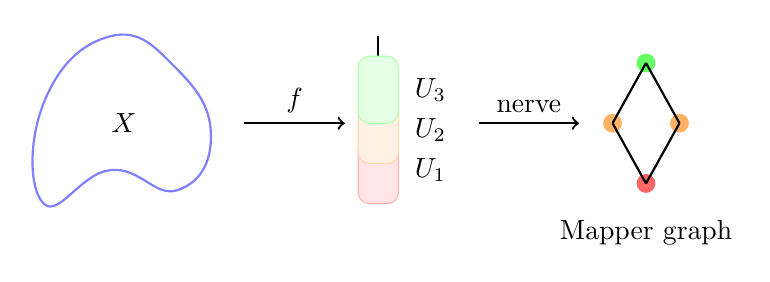
\begin{tikzpicture}[scale=0.85]
  % Data space
  \draw[thick, blue!50] plot[smooth cycle, tension=0.8]
    coordinates {(0,0) (1,0.5) (2,0.2) (2.5,1) (2,2) (1,2.5) (0,1.5)};
  \node at (1.2, 1.2) {$X$};
  \draw[->, thick] (3, 1.2) -- (4.5, 1.2) node[midway, above] {$f$};

  % Filter image
  \draw[thick] (5, 0) -- (5, 2.5);
  \draw[red!30, fill=red!10, rounded corners] (4.7, 0) rectangle (5.3, 1.0);
  \draw[orange!30, fill=orange!10, rounded corners] (4.7, 0.6)
    rectangle (5.3, 1.6);
  \draw[green!30, fill=green!10, rounded corners] (4.7, 1.2)
    rectangle (5.3, 2.2);
  \node[right] at (5.4, 0.5) {$U_1$};
  \node[right] at (5.4, 1.1) {$U_2$};
  \node[right] at (5.4, 1.7) {$U_3$};

  \draw[->, thick] (6.5, 1.2) -- (8, 1.2) node[midway, above] {nerve};

  % Mapper graph
  \fill[red!60] (9, 0.3) circle (4pt);
  \fill[orange!60] (8.5, 1.2) circle (4pt);
  \fill[orange!60] (9.5, 1.2) circle (4pt);
  \fill[green!60] (9, 2.1) circle (4pt);
  \draw[thick] (9, 0.3) -- (8.5, 1.2);
  \draw[thick] (9, 0.3) -- (9.5, 1.2);
  \draw[thick] (8.5, 1.2) -- (9, 2.1);
  \draw[thick] (9.5, 1.2) -- (9, 2.1);
  \node[below] at (9, -0.1) {Mapper graph};
\end{tikzpicture}
\end{center}

% ============================================================
\section{Parameter Choices}
% ============================================================

\subsection{Filter Function}

\begin{definition}[Common Filter Functions]
\begin{itemize}
  \item \textbf{Coordinate}: projection onto an axis, a principal
        component.
  \item \textbf{Eccentricity}: $f(x) = \left(\frac{1}{n}
        \sum_{i=1}^n d(x, x_i)^p\right)^{1/p}$.
  \item \textbf{Density}: kernel density estimation (KDE),
        $k$-nearest neighbors.
  \item \textbf{Distance to $k$-th neighbor}: isolation measure.
  \item \textbf{Learned functions}: t-SNE components, UMAP,
        autoencoder.
\end{itemize}
\end{definition}

\subsection{Cover}

\begin{definition}[Interval Cover]
For a filter function $f : X \to \R$, a standard cover is defined by:
\begin{itemize}
  \item $n_{\mathrm{int}}$: number of intervals.
  \item $p_{\mathrm{ov}}$: overlap percentage ($0 < p_{\mathrm{ov}} < 1$).
\end{itemize}
Each interval has width
$w = \frac{\max f - \min f}{n_{\mathrm{int}} - (n_{\mathrm{int}} - 1) p_{\mathrm{ov}}}$
and the intervals are:
\[
  U_k = [\min f + k(1 - p_{\mathrm{ov}})w,\;
         \min f + k(1 - p_{\mathrm{ov}})w + w].
\]
\end{definition}

\begin{warning}[title=\textbf{Parameter Sensitivity}]
Mapper's output depends strongly on the choice of filter function,
number of intervals, overlap, and clustering algorithm. It is essential
to vary these parameters and assess the robustness of the resulting
graph.
\end{warning}

% ============================================================
\section{Implementation with KeplerMapper}
% ============================================================

\begin{codeblock}[title=\textbf{Mapper with KeplerMapper}]
\begin{minted}{python}
import numpy as np
import kmapper as km
from sklearn.datasets import make_circles
from sklearn.cluster import DBSCAN

# Data: two concentric circles
X, y = make_circles(n_samples=500, noise=0.05, factor=0.5)

# Initialize Mapper
mapper = km.KeplerMapper(verbose=1)

# Filter function: projection onto first coordinate
lens = mapper.fit_transform(X, projection=[0])

# Build Mapper graph
graph = mapper.map(
    lens, X,
    cover=km.Cover(n_cubes=15, perc_overlap=0.4),
    clusterer=DBSCAN(eps=0.3, min_samples=5)
)

# HTML visualization
mapper.visualize(
    graph,
    path_html="mapper_circles.html",
    title="Mapper: Concentric Circles",
    color_values=y
)
print(f"Number of nodes: {len(graph['nodes'])}")
print(f"Number of edges: {len(graph['links'])}")
\end{minted}
\end{codeblock}

% ============================================================
\section{Mapper with GUDHI}
% ============================================================

\begin{codeblock}[title=\textbf{Manual Mapper Construction}]
\begin{minted}{python}
import numpy as np
from sklearn.cluster import DBSCAN
from sklearn.neighbors import KernelDensity

X = np.random.randn(200, 3)

# Filter: density
kde = KernelDensity(bandwidth=0.5)
kde.fit(X)
f_values = kde.score_samples(X)

# Cover
n_intervals = 10
overlap = 0.3
f_min, f_max = f_values.min(), f_values.max()
width = (f_max - f_min) / (n_intervals - (n_intervals-1) * overlap)

clusters_all = []
for k in range(n_intervals):
    start = f_min + k * (1 - overlap) * width
    end = start + width
    mask = (f_values >= start) & (f_values <= end)
    if mask.sum() < 2:
        continue
    X_local = X[mask]
    db = DBSCAN(eps=0.5, min_samples=3).fit(X_local)
    labels = db.labels_
    for l in set(labels):
        if l == -1:
            continue
        idx = np.where(mask)[0][labels == l]
        clusters_all.append(set(idx.tolist()))

# Build edges (non-empty intersection)
edges = []
for i in range(len(clusters_all)):
    for j in range(i+1, len(clusters_all)):
        if clusters_all[i] & clusters_all[j]:
            edges.append((i, j))

print(f"Nodes: {len(clusters_all)}, Edges: {len(edges)}")
\end{minted}
\end{codeblock}

% ============================================================
\section{Theoretical Foundations}
% ============================================================

\begin{theorem}[Mapper Convergence --- Carri\`ere, Oudot, 2018]
Under regularity conditions on $f$ and $X$, as the number of points
$n \to \infty$ and the cover parameters are chosen appropriately, the
Mapper graph converges (in the functional interleaving distance) to the
Reeb graph of $(X, f)$.
\end{theorem}

\begin{definition}[Functional Interleaving Distance]
Let $\mathcal{R}_1$ and $\mathcal{R}_2$ be two Reeb graphs. The
\emph{functional interleaving distance} is:
\[
  d_{\mathrm{FI}}(\mathcal{R}_1, \mathcal{R}_2) =
  \inf_{\varepsilon} \{\varepsilon \geq 0 :
  \mathcal{R}_1 \text{ and } \mathcal{R}_2 \text{ are }
  \varepsilon\text{-interleaved}\}.
\]
\end{definition}

% ============================================================
\section{Multidimensional Mapper}
% ============================================================

\begin{definition}[2D Mapper]
When the filter function is $f : X \to \R^2$, the cover is a grid of
overlapping rectangles in $\R^2$. The result is a simplicial complex of
potentially dimension $\geq 2$ (not just a graph).
\end{definition}

\begin{codeblock}[title=\textbf{2D Mapper with KeplerMapper}]
\begin{minted}{python}
import kmapper as km
import numpy as np
from sklearn.datasets import make_swiss_roll
from sklearn.cluster import DBSCAN

# Data: Swiss roll
X, color = make_swiss_roll(n_samples=1000, noise=0.5)

mapper = km.KeplerMapper()

# 2D filter: first and third coordinates
lens = mapper.fit_transform(X, projection=[0, 2])

graph = mapper.map(
    lens, X,
    cover=km.Cover(n_cubes=10, perc_overlap=0.3),
    clusterer=DBSCAN(eps=2.0, min_samples=5)
)

mapper.visualize(graph, path_html="mapper_swiss_roll.html",
                 color_values=color, title="Swiss Roll Mapper")
\end{minted}
\end{codeblock}

% ============================================================
\section{Famous Applications of Mapper}
% ============================================================

\subsection{Breast Cancer (Lum et al., 2013)}
The seminal biological study using Mapper revealed subgroups in breast
cancer gene expression data that had not been detected by classical
clustering methods.

\subsection{Basketball Player Analysis (Lum et al., 2013)}
Mapper was applied to NBA player statistics, revealing a ``Y''-shaped
structure corresponding to the three main roles (guard, forward,
center).

\subsection{Type 2 Diabetes (Li et al., 2015)}
Mapper identified three distinct subtypes of type~2 diabetes from
clinical data, with therapeutic implications.

% ============================================================
\section{Ball Mapper}
% ============================================================

\begin{definition}[Ball Mapper --- D\l{}otko, 2019]
\emph{Ball Mapper} is a simplified variant of Mapper where:
\begin{enumerate}
  \item Fix a radius $\varepsilon > 0$.
  \item Select a subset of landmark points $L \subset X$ (by farthest
        point sampling).
  \item Nodes are the balls $B(l, \varepsilon)$ for $l \in L$.
  \item Two nodes are connected if their balls share common data points.
\end{enumerate}
Advantage: no need to choose a filter function.
\end{definition}

% ============================================================
\section{Exercises}
% ============================================================

\begin{exercise}
Apply Mapper to the iris dataset
(\texttt{sklearn.datasets.load\_iris}) with different filter functions
(PCA, eccentricity, density). Compare the resulting graphs.
\end{exercise}

\begin{exercise}
Study the effect of the number of intervals and overlap percentage on
the Mapper graph. For a noisy circle, determine parameters that produce
a cyclic graph.
\end{exercise}

\begin{exercise}
Implement Ball Mapper in Python and apply it to a 3D point cloud.
\end{exercise}

\begin{exercise}
Show that if the cover is sufficiently fine and the clustering algorithm
is exact, the Mapper graph is an approximation of the Reeb graph of
$(X, f)$.
\end{exercise}

\begin{exercise}
Download a real-world dataset (e.g., genomic expression data) and apply
Mapper to identify subgroups. Interpret the resulting graph.
\end{exercise}
